\pgfplotsset{
x tick label style={/pgf/number format/fixed,
        /pgf/number format/precision=1,
		font=\tiny},
y tick label style={/pgf/number format/fixed,
        /pgf/number format/precision=1,
		font=\tiny},
y label style={font=\tiny},
x label style={font=\tiny},
legend style={font=\fontsize{10}{5}\selectfont},
   }%
\begin{tabular}{ll}
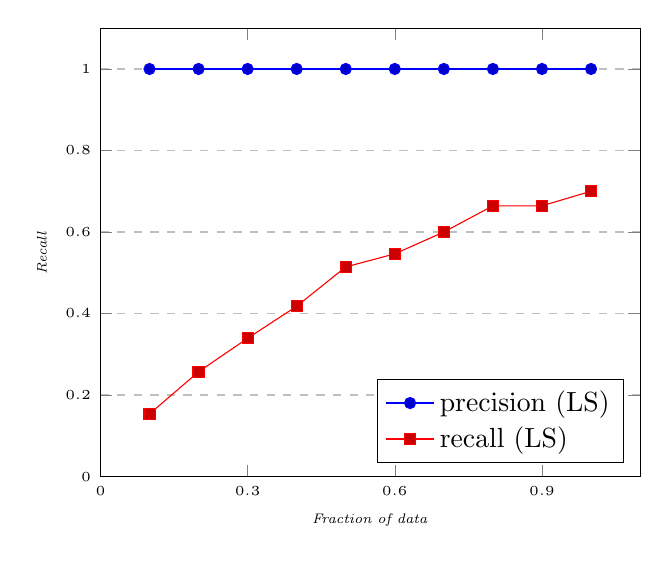
\begin{tikzpicture}
 \begin{axis}[
   xmax=1.1,xmin=0,
   ymin= 0,ymax=1.1,
   xlabel=\emph{Fraction of data},
ylabel=\emph{Recall},
   xtick={0,0.3,0.6,...,1},
   ytick={0,0.2,0.4,...,1},
legend style={legend pos=south east},
 ymajorgrids=true,
    grid style=dashed,
legend cell align=left,
   ]
\addplot coordinates{
(0.1,1.0)
(0.2,1.0)
(0.30000000000000004,1.0)
(0.4,1.0)
(0.5,1.0)
(0.6,1.0)
(0.7,1.0)
(0.7999999999999999,1.0)
(0.8999999999999999,1.0)
(0.9999999999999999,1.0)
};

\addplot coordinates{
(0.1,0.15357142857142858)
(0.2,0.2571428571428571)
(0.30000000000000004,0.3392857142857143)
(0.4,0.41785714285714287)
(0.5,0.5142857142857142)
(0.6,0.5464285714285714)
(0.7,0.6)
(0.7999999999999999,0.6642857142857143)
(0.8999999999999999,0.6642857142857143)
(0.9999999999999999,0.7)
};
    \legend{precision (LS), recall (LS)}    \end{axis}
    \end{tikzpicture}&
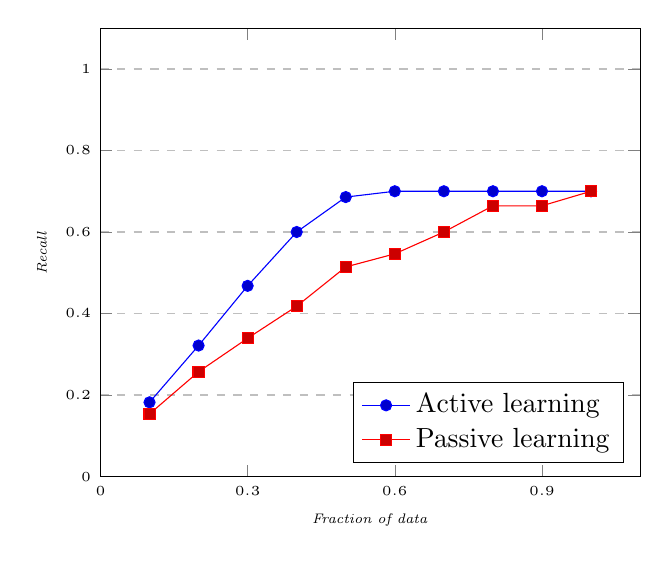
\begin{tikzpicture}
    \begin{axis}[
   xmax=1.1,xmin=0,
   ymin= 0,ymax=1.1,
   xlabel=\emph{Fraction of data},
ylabel=\emph{Recall},
   xtick={0,0.3,0.6,...,1},
   ytick={0,0.2,0.4,...,1},
legend style={legend pos=south east},
 ymajorgrids=true,
    grid style=dashed,
legend cell align=left,
   ]
\addplot coordinates{
(0.1,0.18214285714285713)
(0.2,0.32142857142857145)
(0.30000000000000004,0.46785714285714286)
(0.4,0.6)
(0.5,0.6857142857142857)
(0.6,0.7)
(0.7,0.7)
(0.7999999999999999,0.7)
(0.8999999999999999,0.7)
(0.9999999999999999,0.7)
};

\addplot coordinates{
(0.1,0.15357142857142858)
(0.2,0.2571428571428571)
(0.30000000000000004,0.3392857142857143)
(0.4,0.41785714285714287)
(0.5,0.5142857142857142)
(0.6,0.5464285714285714)
(0.7,0.6)
(0.7999999999999999,0.6642857142857143)
(0.8999999999999999,0.6642857142857143)
(0.9999999999999999,0.7)
};



    %\legend{Independent examples, Random examples}
    \legend{Active learning, Passive learning}
  \end{axis}
    \end{tikzpicture}
\end{tabular}